\section{Feedbacks}
\begin{frame}{Oque estão achando?}
    \begin{figure}
        \centering
        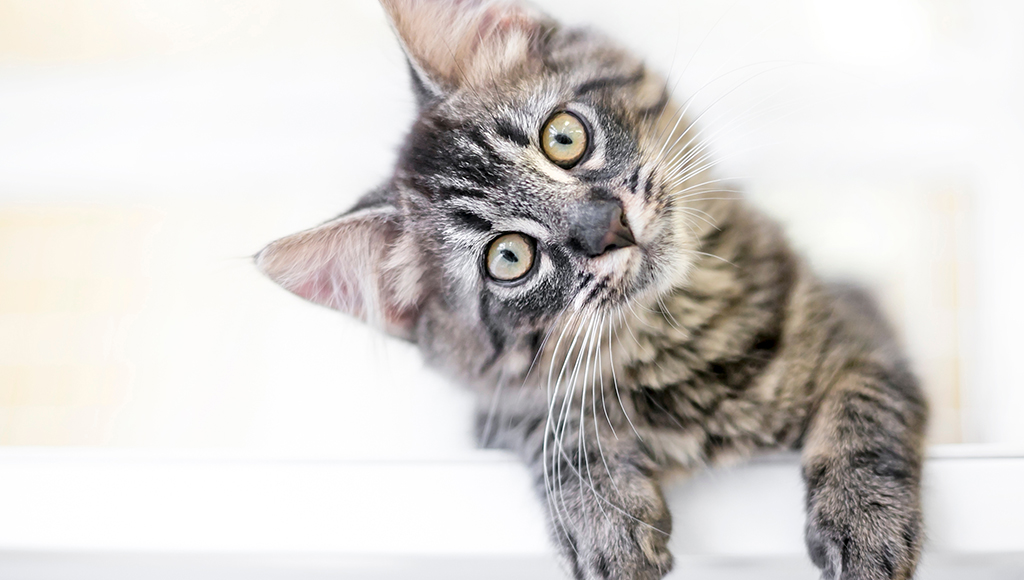
\includegraphics[width=1\linewidth]{figuras/curious.jpg}
    \end{figure}
\end{frame}

\section{Introdução}


\begin{frame}{Introdução}
Frequentemente no computador a \textbf{entrada de dados} é  feita pelo teclado e a \textbf{saída de dados} é feita em tela

\begin{figure}
    \centering
    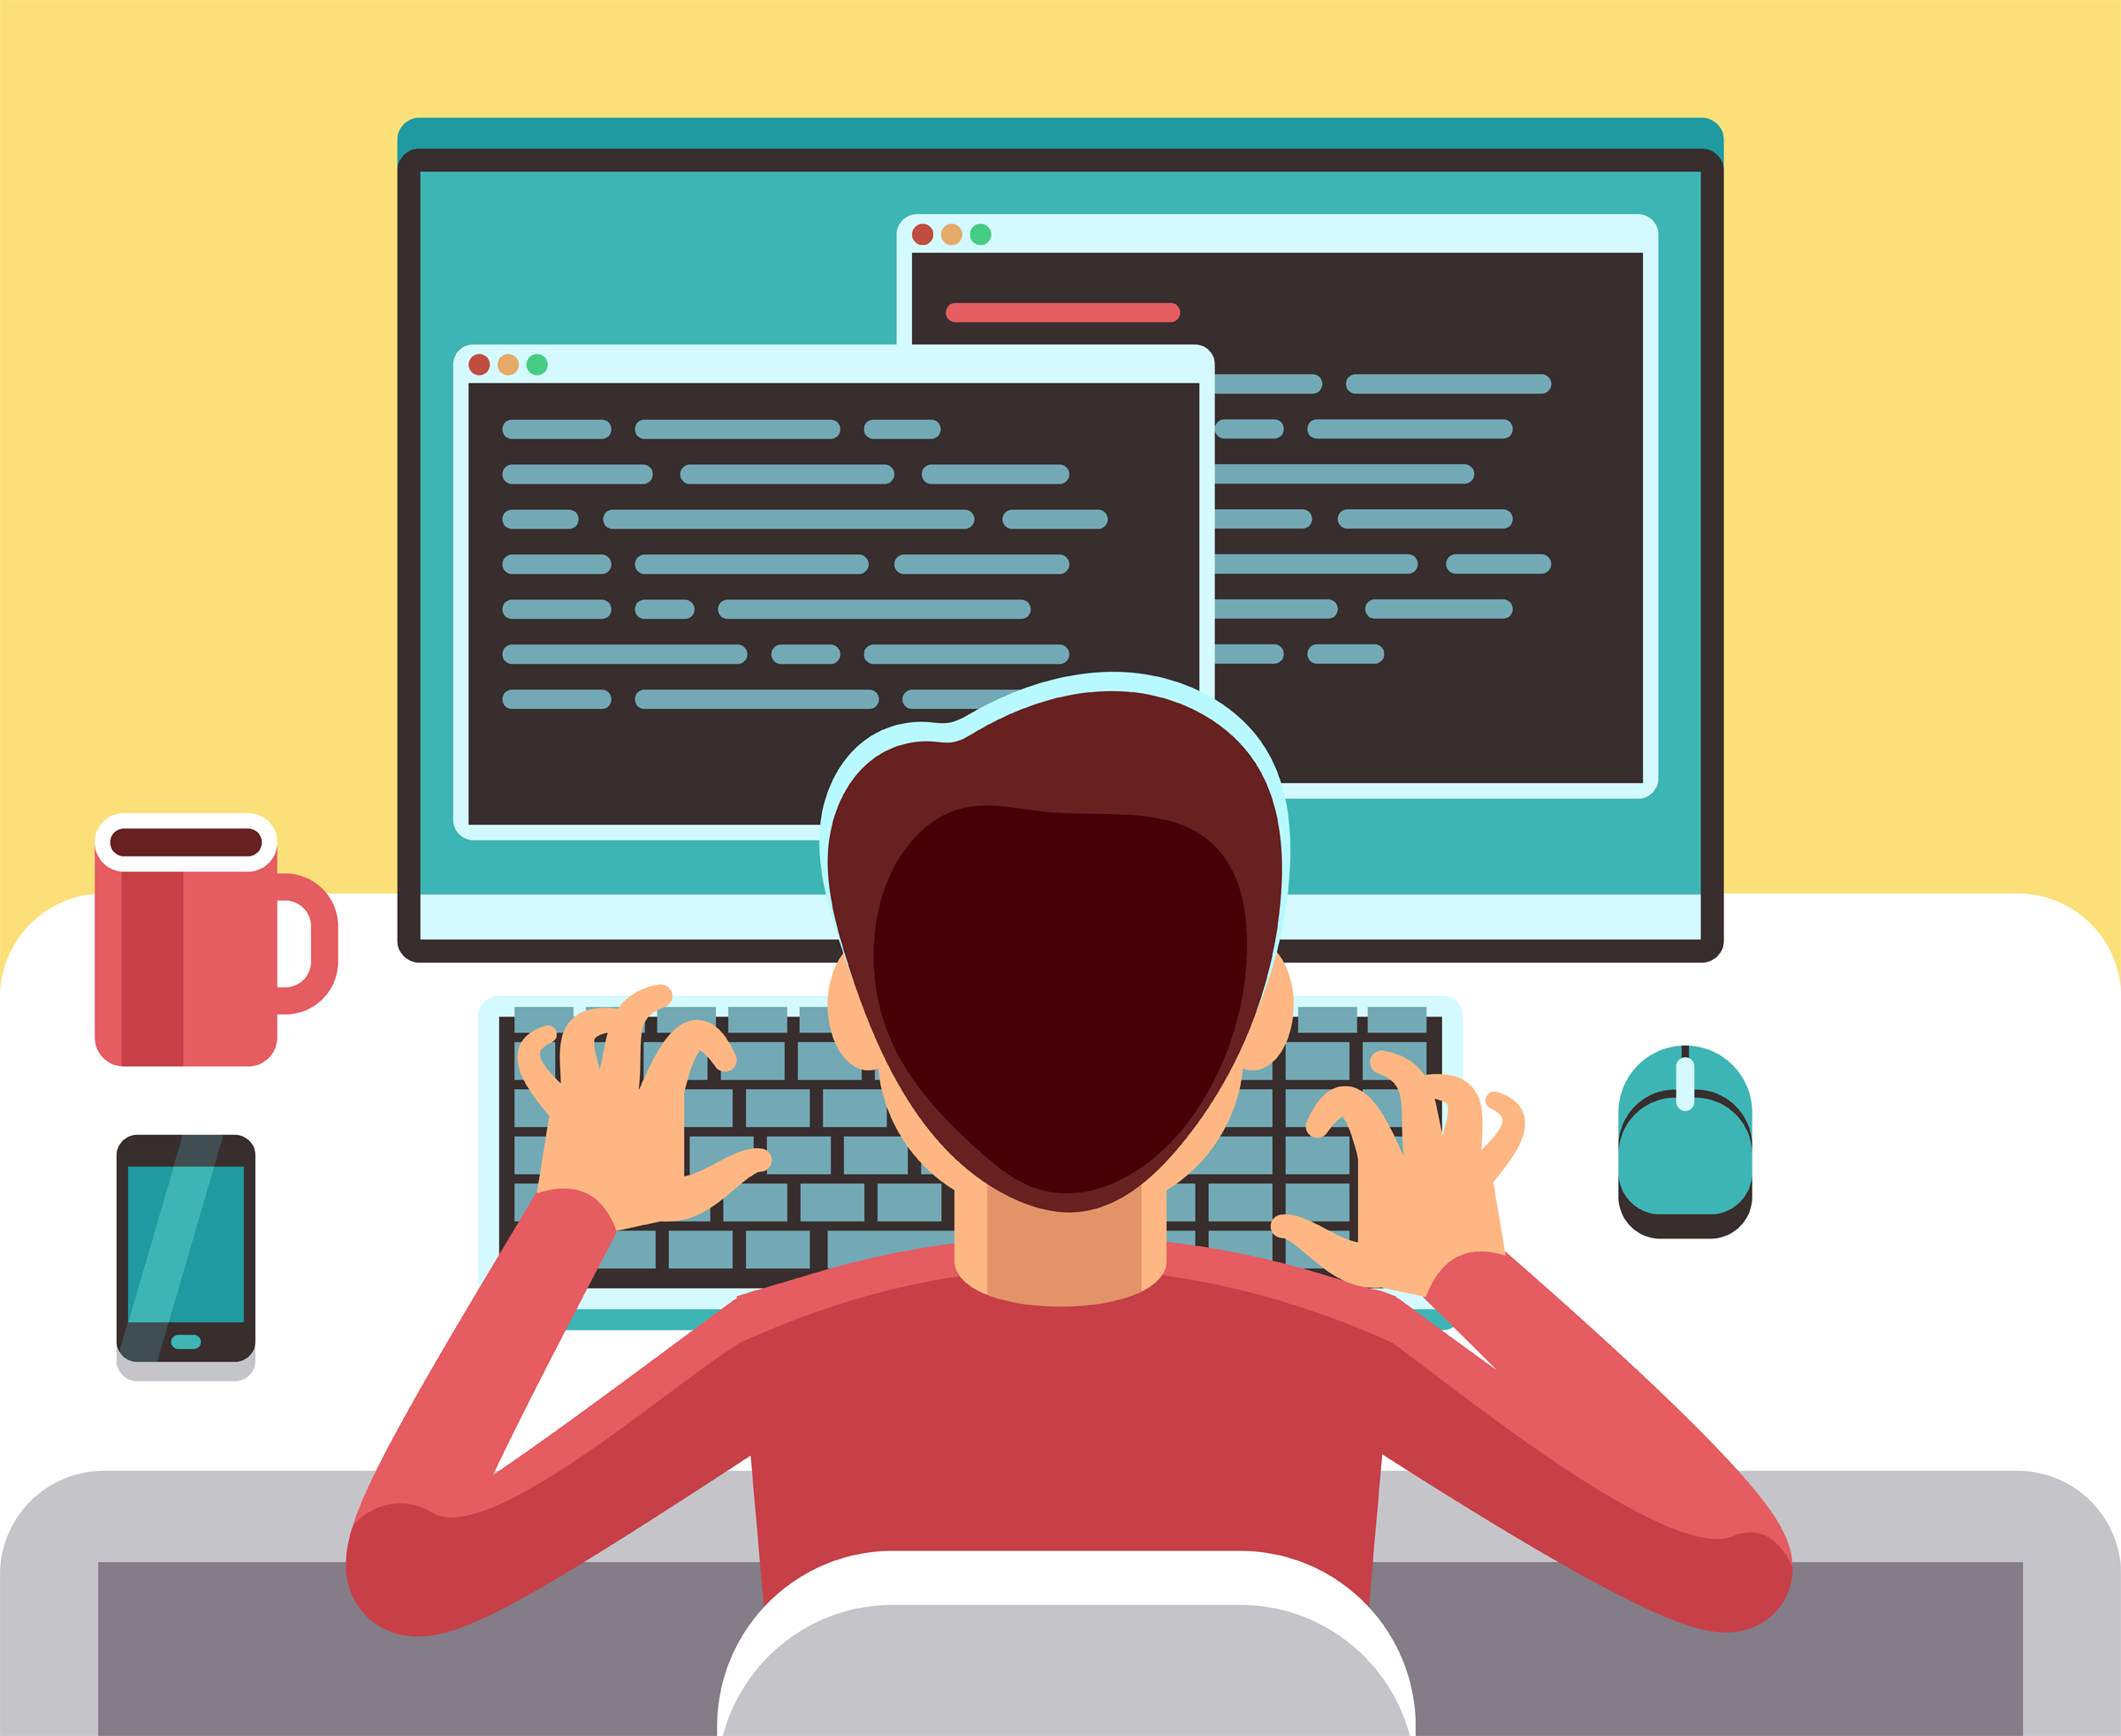
\includegraphics[width=0.7\linewidth]{figuras/ilust.png}
\end{figure}
\end{frame}




\begin{frame}{Introdução}
As vezes a \textbf{saída de dados} na tela não é a melhor opção:
\begin{itemize}
    \item Seria conveniente gravar em \textbf{um arquivo} a lista de produtos necessitando reposição de estoque
\end{itemize}
    \begin{figure}
        \centering
        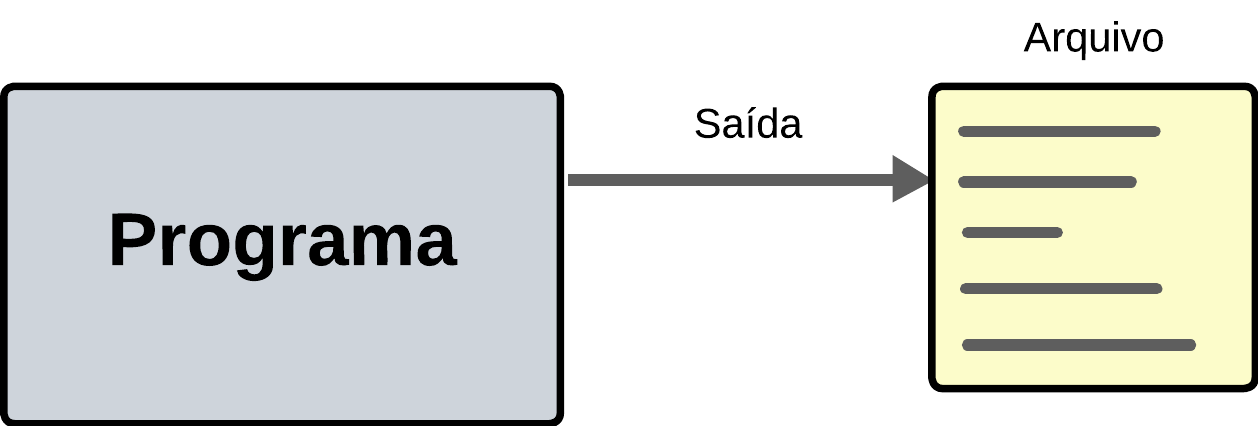
\includegraphics[width=0.75\linewidth]{figuras/arqpro.png}
    \end{figure}
\end{frame}

\begin{frame}{Introdução}
\begin{itemize}
    \item Os \textbf{programas} de computador \textbf{trabalham com arquivos}
    \begin{itemize}
        \item \textbf{Documentos, planilhas, apresentações, imagens, vídeos, sons}, etc.
são armazenados e manipulados a partir de arquivos
        \item \textbf{Compiladores} leem o arquivo fonte de um programa e
geram um arquivo executável
    \end{itemize}
    \item Um \textbf{arquivo} é um \textbf{conjunto de bits} guardado em algum dispositivo de armazenamento permanente. \\(SSD, HD, Pen-Drive, etc.)
\end{itemize}
    
\end{frame}


\begin{frame}{Introdução}
\begin{itemize}
    \item O \textbf{sistema operacional} se encarrega de gerenciar os arquivos
    \begin{itemize}
        \item Saber a sua localização no disco
        \item Guardar informações sobre o arquivo (Tamanho, datas de criação e modificação, permissões, etc.)
    \end{itemize}
    \item Como programador estamos interessados em \textbf{conectar um programa a um arquivo} para:
    \begin{itemize}
        \item Ler informações do arquivo
        \item Gravar informações no arquivo
    \end{itemize}
\end{itemize}
    
\end{frame}

\begin{frame}{Introdução}
\begin{itemize}
    \item Para um programador os arquivos se dividem em:
    \begin{itemize}
        \item \textbf{Arquivos de texto}
        \item \textbf{Arquivos binários}
    \end{itemize}
\end{itemize}
    
\end{frame}


\begin{frame}{Introdução}
\begin{itemize}
    \item Para um programador os arquivos se dividem em:
    \begin{itemize}
        \item \textbf{Arquivos de texto}
        \item \textbf{Arquivos binários}
    \end{itemize}
\end{itemize}
\begin{figure}
    \centering
    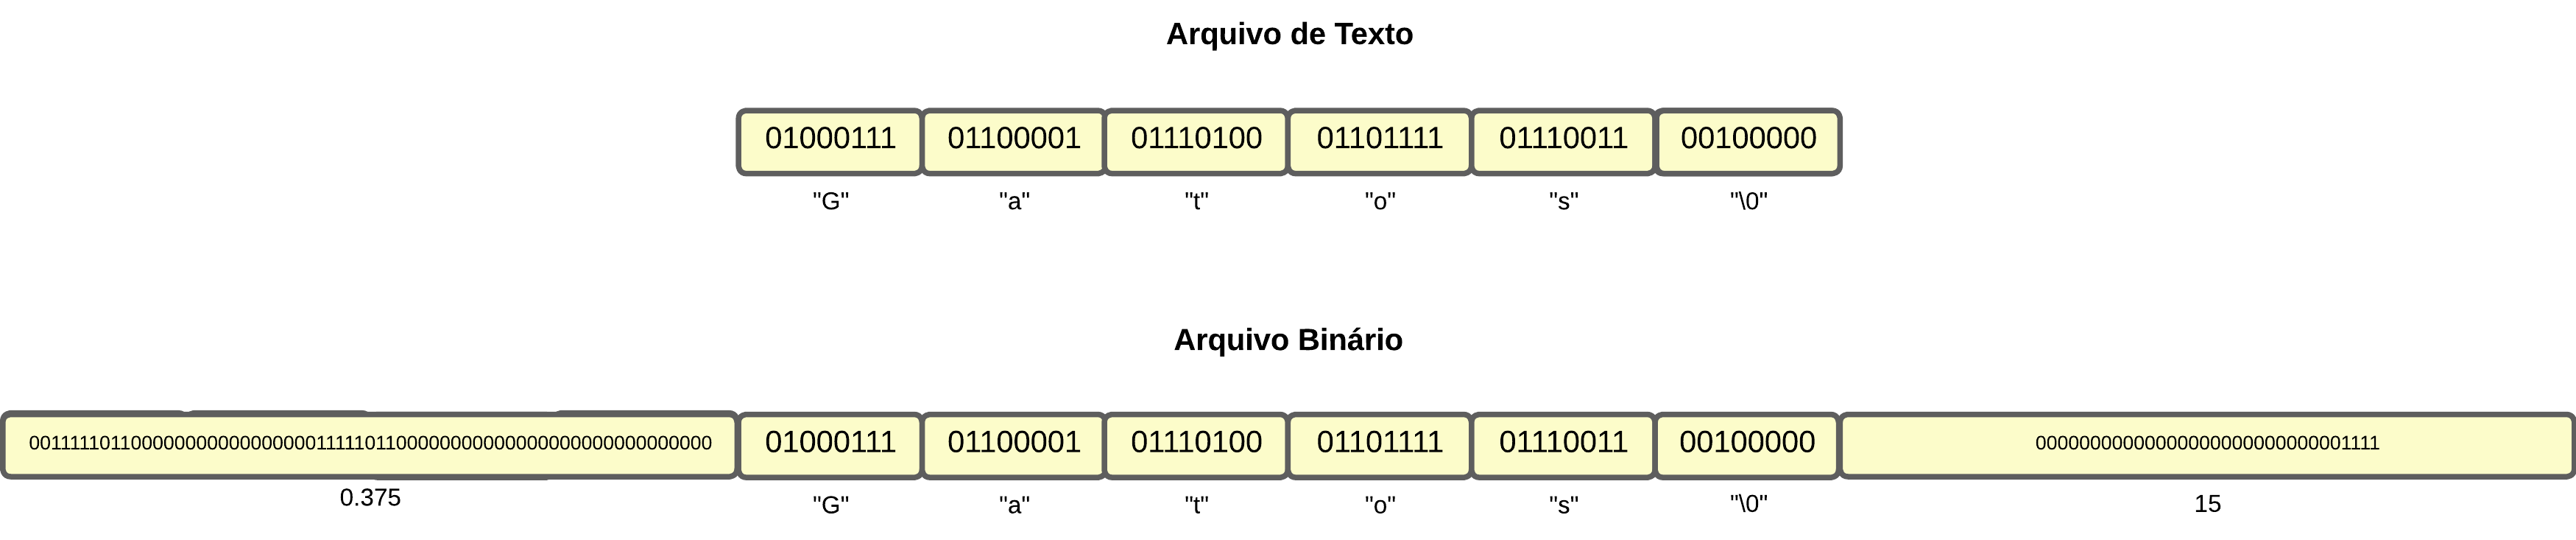
\includegraphics[width=1\linewidth]{figuras/arqTyp.png}
\end{figure}
\end{frame}




\begin{frame}{Arquivos de Texto}
\begin{itemize}
    \item Uma sequência de bits em que \textbf{n bits representam um caractere}
    \item Na codificação \textbf{ASCII} um caractere são \textbf{8 bits}
    \item Em \textbf{Unicode} um caractere tem de \textbf{8 a 32 bits}
    \begin{itemize}
        \item Existem várias codificações (UTF-8, UTF-16, UTF-32)\\
    \end{itemize}
\end{itemize}
\begin{figure}
    \centering
    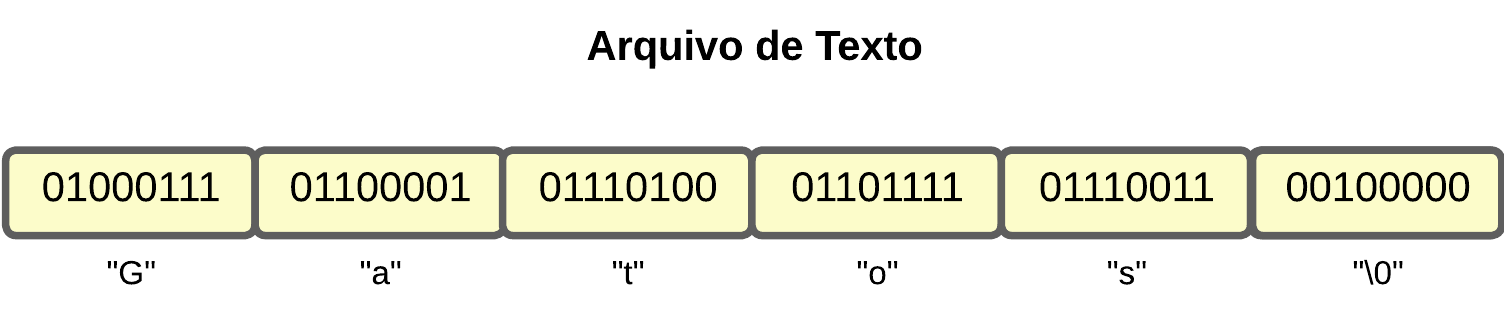
\includegraphics[width=1\linewidth]{figuras/textArq.png}
\end{figure}
\end{frame}


\begin{frame}{Arquivos Binários}
\begin{itemize}
    \item Uma sequência de bits em que um conjunto de \textbf{n bits representa} uma informação na sua \textbf{forma nativa} (inteira, ponto-flutuante, caractere, etc.)\\
\end{itemize}
\begin{figure}
    \centering
    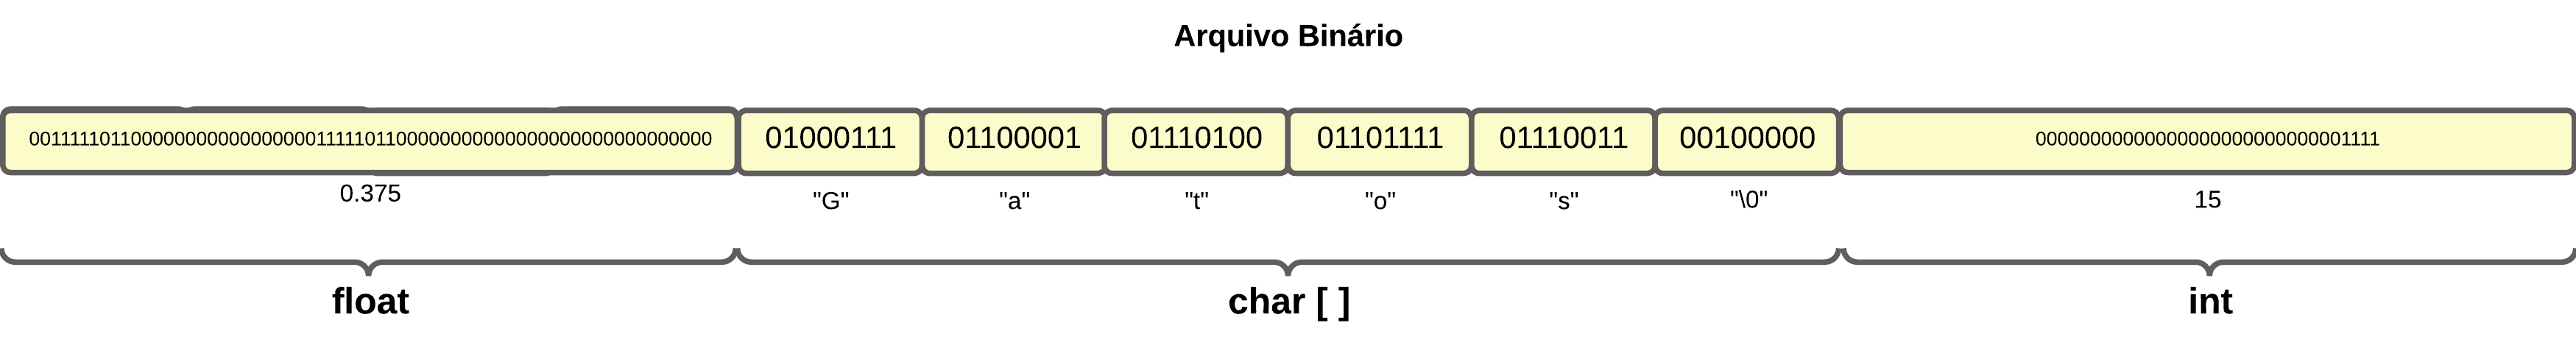
\includegraphics[width=1\linewidth]{figuras/binArq.png}
\end{figure}
\end{frame}


\begin{frame}{Diferença entre Arquivos Binários e de Texto}
\begin{figure}
    \centering
    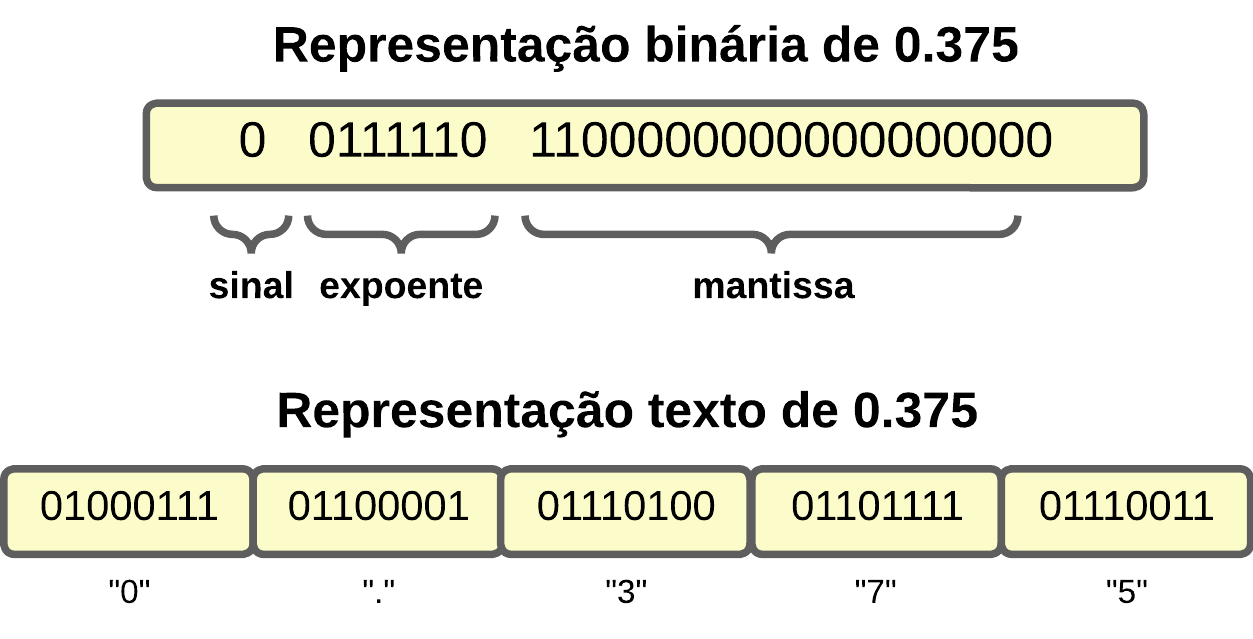
\includegraphics[width=1\linewidth]{figuras/difArq.png}
\end{figure}
\end{frame}


\begin{frame}{Diferença entre Arquivos Binários e de Texto}
A entrada e saída em arquivos texto é muito parecida com a
entrada e saída feita no terminal de comandos
\begin{figure}
    \centering
    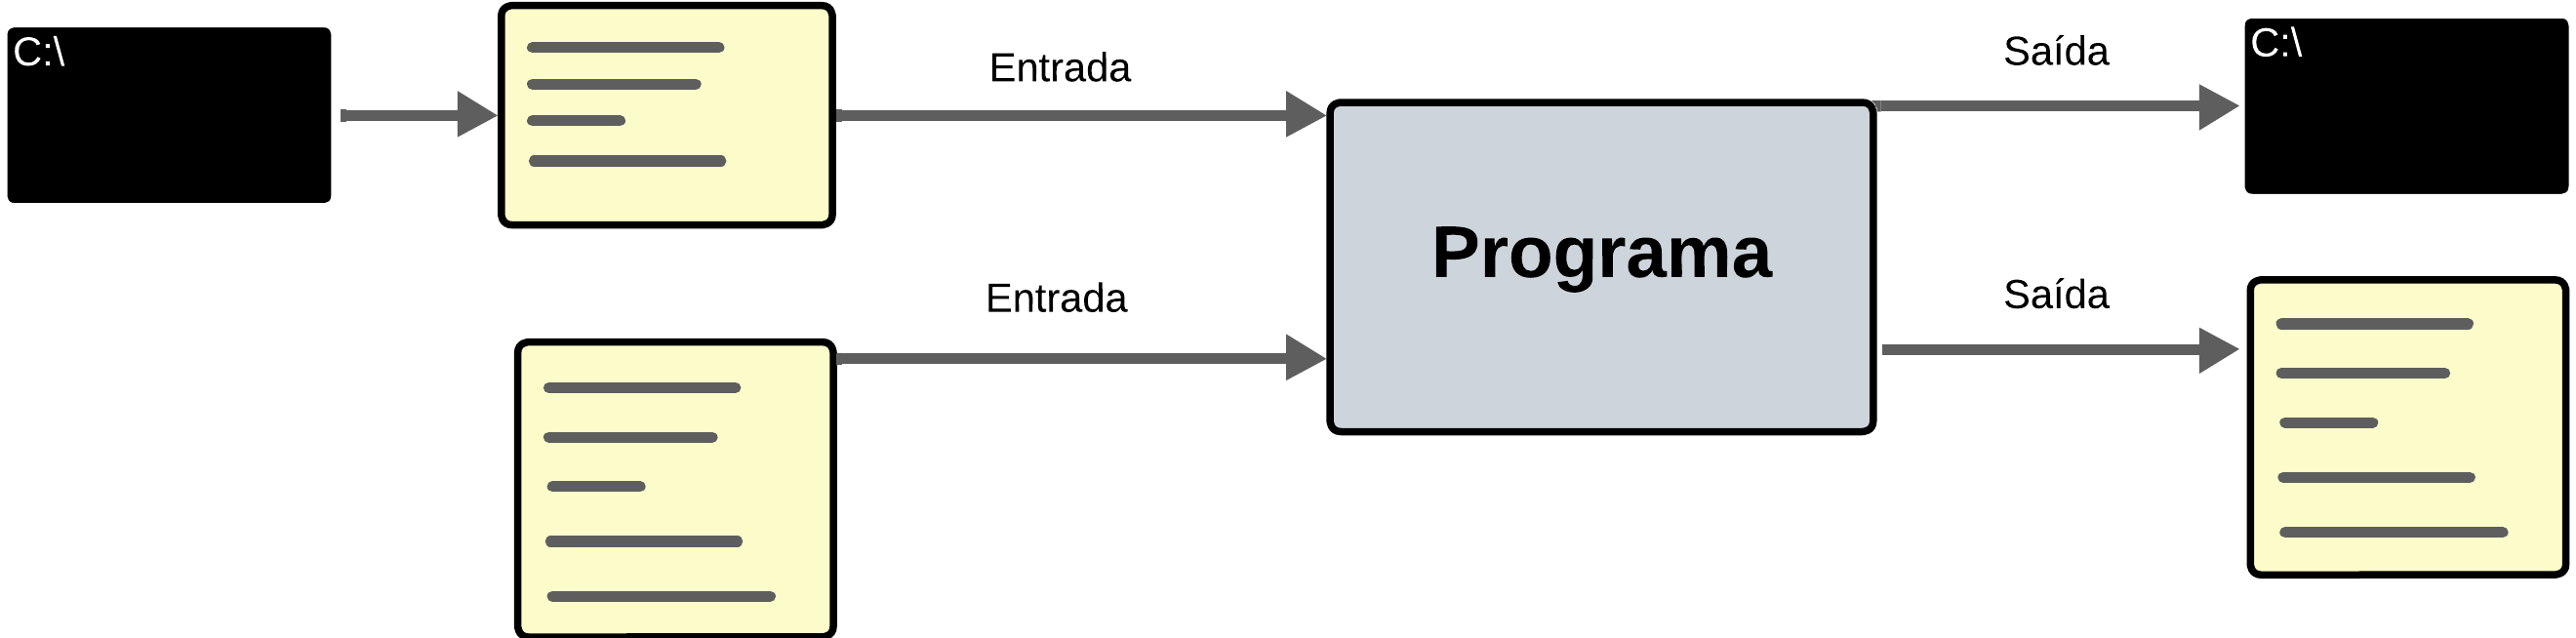
\includegraphics[width=1\linewidth]{figuras/difArq2.png}
\end{figure}
\end{frame}

\section{Arquivo Texto}

\begin{frame}{Saída em Tela}
Exemplo de Saída em Tela:
    \begin{figure}
        \centering
        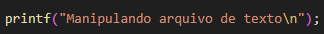
\includegraphics[width=1\linewidth]{figuras/SaidaTela.png}\\
        
    \end{figure}
    \begin{figure}
        \centering
        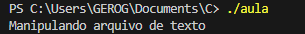
\includegraphics[width=1\linewidth]{figuras/saidaTela2.png}
    \end{figure}
\end{frame}



\begin{frame}{Saída em Arquivos}
Como acessamos um arquivo em C?
    \begin{figure}
        \centering
        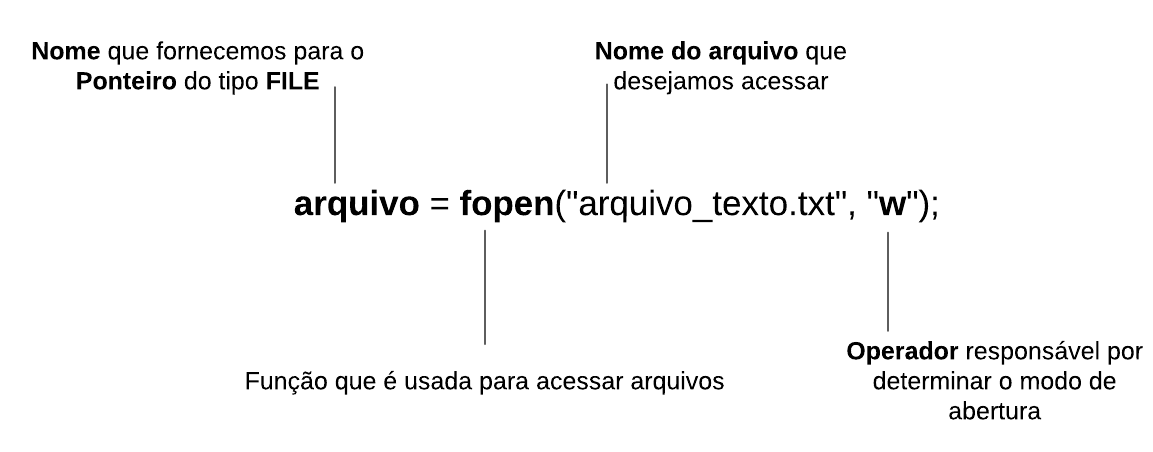
\includegraphics[width=1\linewidth]{figuras/ArqOpen.png}
    \end{figure}
\end{frame}

\begin{frame}{Operadores Utilizados para Arquivos Texto}
    \begin{table}[h]
    \centering
    \begin{tabular}{|c|l|}
        \hline
        \textbf{Modo} & \textbf{Descrição} \\
        \hline
        \texttt{"\textbf{r}"}   & Abre um arquivo para leitura. \\
                        & Se o arquivo não existir, retorna \texttt{NULL}. \\
        \hline
        \texttt{"\textbf{w}"}   & Cria um arquivo para escrita. \\
                        & Se o arquivo já existir, ele será apagado. \\
        \hline
        \texttt{"\textbf{a}"}   & Abre um arquivo para adicionar dados ao final. \\
                        & Não altera dados existentes no arquivo. \\
        \hline
        \texttt{"\textbf{r+}"}  & Abre um arquivo para leitura e escrita. \\
                        & O arquivo deve existir previamente. \\
        \hline
        \texttt{"\textbf{w+}"}  & Cria um arquivo para leitura e escrita. \\
                        & Se o arquivo já existir, ele será apagado. \\
        \hline
        \texttt{"\textbf{a+}"}  & Abre um arquivo para leitura e escrita. \\
                        & Não apaga dados existentes no arquivo. \\
        \hline
    \end{tabular}
    \caption{Modos de abertura de arquivos de texto em C}
    \label{tab:modos_arquivo_texto}
\end{table}
\end{frame}


\begin{frame}{Diferença dos Operados com e sem o +}
Resumo das Diferenças:
\begin{itemize}
    \item Sem o +: O arquivo é aberto apenas para leitura ou apenas para escrita.
    \item Com o +: O arquivo é aberto para leitura e escrita simultaneamente. Isso significa que você pode modificar o conteúdo do arquivo e também ler ao mesmo tempo.
\end{itemize}
\end{frame}


\begin{frame}{Saída em Arquivos}
Exemplo de Saída em Arquivo:
    \begin{figure}
        \centering
        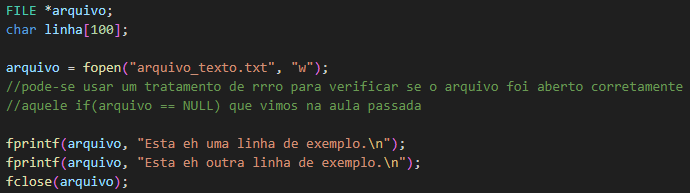
\includegraphics[width=1\linewidth]{figuras/saidaArq.png}
    \end{figure}
\end{frame}

\begin{frame}{Saída em Arquivos}
Exemplo de Saída em Arquivo:
    \begin{figure}
        \centering
        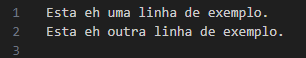
\includegraphics[width=1\linewidth]{figuras/saidaArq2.png}
    \end{figure}
\end{frame}

\begin{frame}{Leitura de Arquivos}
    A leitura de arquivos é muito semelhante à criação de arquivos
    \begin{figure}
        \centering
        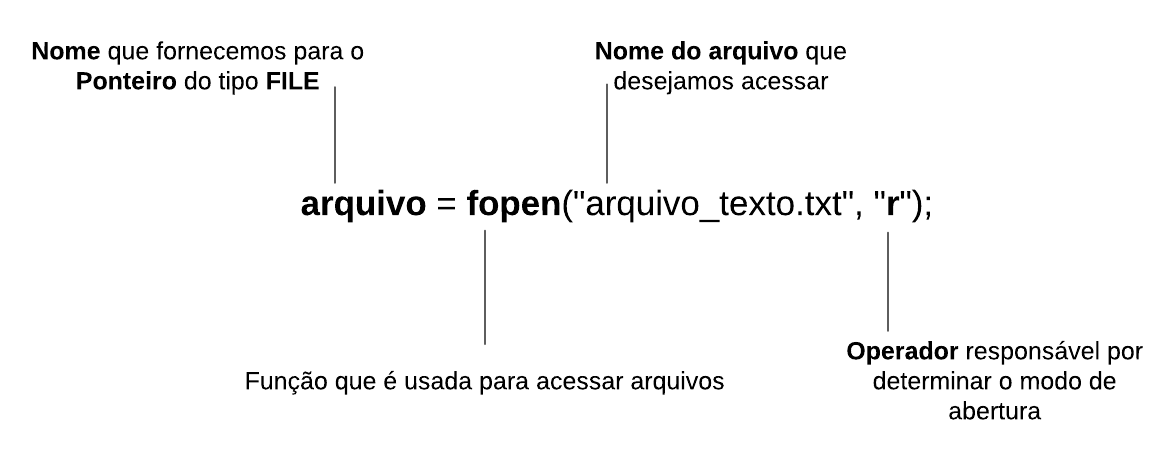
\includegraphics[width=1\linewidth]{figuras/ArqRead0.png}
    \end{figure}
\end{frame}

\begin{frame}{Leitura de Arquivos}
\begin{itemize}
    \item Utilizamos o operador \textbf{fgetc(arquivo)} para ler um caractere por vez
    \item Utilizamos o operador \textbf{EOF} para indicar que queremos ler até o final do arquivo (End Of File)
\end{itemize}

    \begin{figure}
        \centering
        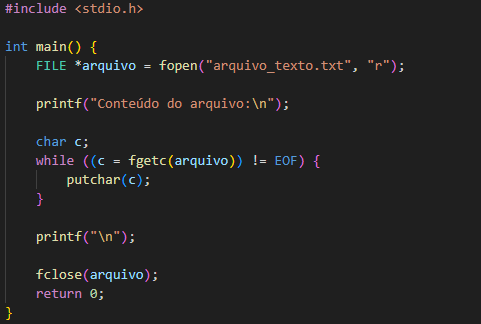
\includegraphics[width=0.5\linewidth]{figuras/ArqRead.png}
    \end{figure}
\end{frame}

\begin{frame}{Leitura de Arquivos}
    Saída da Leitura do arquivo:
    \begin{figure}
        \centering
        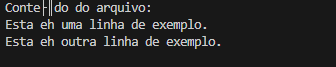
\includegraphics[width=1\linewidth]{figuras/ArqRead2.png}
    \end{figure}
\end{frame}

\begin{frame}{Leitura de Arquivos}
Outro Exemplo de Leitura de Arquivo:
\begin{itemize}
    \item Agora utilizando o operador \textbf{fgets} para ler uma linha inteira do arquivo
\end{itemize}
    \begin{figure}
        \centering
        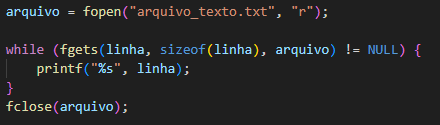
\includegraphics[width=1\linewidth]{figuras/ArqLeitura.png}
    \end{figure}
\end{frame}

\begin{frame}{Leitura de Arquivos}
Outro Exemplo de Leitura de Arquivo:
    \begin{figure}
        \centering
        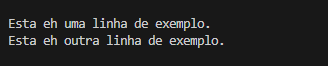
\includegraphics[width=1\linewidth]{figuras/ArqLeitura2.png}
    \end{figure}
\end{frame}

\begin{frame}{Leitura de Arquivos Formatados}
Primeiramente podemos criar manualmente um arquivo .txt para ser lido:
\begin{figure}
    \centering
    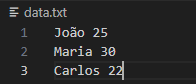
\includegraphics[width=0.6\linewidth]{figuras/ArqForm1.png}
\end{figure}

\end{frame}

\begin{frame}{Leitura de Arquivos Formatados}
A função \textbf{fscanf()} funciona como \textbf{scanf()}, mas lê diretamente do arquivo.
\begin{figure}
    \centering
    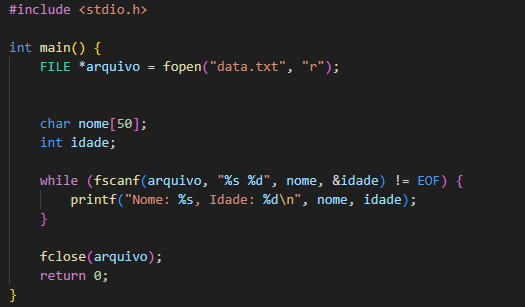
\includegraphics[width=0.65\linewidth]{figuras/ArqForm2.png}
\end{figure}

fscanf(arquivo, "\%s \%d", nome, \&idade) → Lê uma string e um número inteiro.
\end{frame}

\begin{frame}{Leitura de Arquivos Formatados}
Saída da Leitura do Arquivo Formatado
\begin{figure}
    \centering
    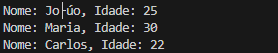
\includegraphics[width=0.75\linewidth]{figuras/ArqForm3.png}
\end{figure}
\end{frame}

\begin{frame}{Recapitulando...}
\begin{itemize}
    \item \textbf{fgetc()} → Lê \textbf{um caractere} por vez.
    \item \textbf{fgets()} → Lê \textbf{uma linha} por vez.
    \item \textbf{fscanf()} → Lê \textbf{dados formatados}.
\end{itemize}
    
\end{frame}
\begin{frame}{Desafio}
\begin{itemize}
    \item Façam um código que \textbf{crie um arquivo} e o \textbf{preencham com informações}
    \item Em seguida \textbf{leiam as informações} que vocês preencheram no arquivo
    \item Em seguida \textbf{alterem alguma informação} que vocês preencheram anteriormente
    \item Leiam novamente o \textbf{arquivo atualizado}
\end{itemize}
\end{frame}

\begin{frame}{Desafio}
Trabalhei com funções para separar melhor as etapas do desafio:
\begin{figure}
    \centering
    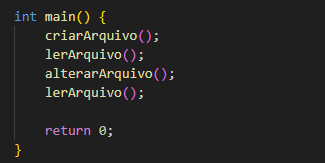
\includegraphics[width=0.75\linewidth]{figuras/Cod1.png}
\end{figure}
\end{frame}

\begin{frame}{Desafio}
Em seguida criei as funções de criar e ler arquivos:
\begin{figure}
    \centering
    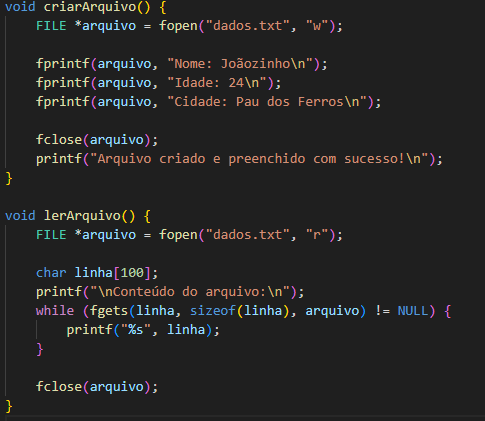
\includegraphics[width=0.5\linewidth]{figuras/Cod2.png}
\end{figure}
\end{frame}

\begin{frame}{Desafio}
Em seguida criei a função de editar arquivos:
\begin{figure}
    \centering
    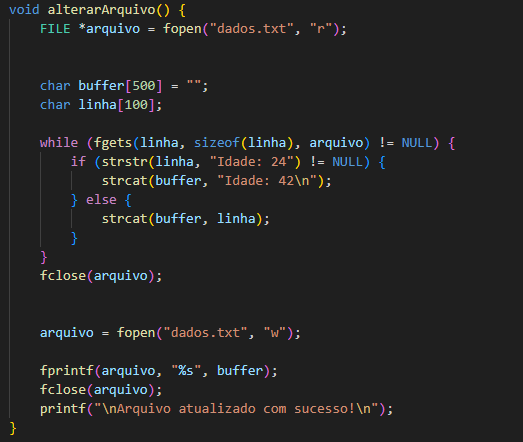
\includegraphics[width=0.5\linewidth]{figuras/Cod3.png}
\end{figure}
\end{frame}


\begin{frame}{Desafio}
Saída do Código:
\begin{figure}
    \centering
    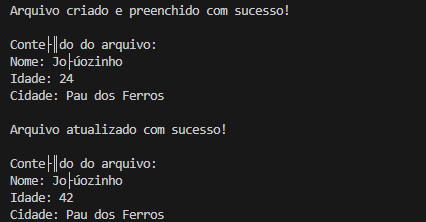
\includegraphics[width=0.9\linewidth]{figuras/Cod4.png}
\end{figure}
\end{frame}


\begin{frame}{Vale Salientar que...}
\begin{itemize}
    \item A \textbf{abertura de arquivo pode falhar} caso o arquivo utilizado seja um arquivo de \textbf{acesso restrito}
    \begin{itemize}
        \item Um \textbf{arquivo já aberto} em outro programa
        \item Um arquivo protegido pelo \textbf{Sistema Operacional}
    \end{itemize}
\end{itemize}
\end{frame}



\section{Arquivo Binário}
\begin{frame}{Introdução a Arquivos Binários}
Temos que:
\begin{itemize}
    \item Um \textbf{arquivo} é um \textbf{conjunto de bits} gravados em algum dispositivo de armazenamento permanente
    \item Os arquivos se dividem em:
    \begin{itemize}
        \item \textbf{Arquivos Texto:} Um conjunto de \textbf{n bits} representa um caractere
        \item \textbf{Arquivos binários:} Um conjunto de \textbf{n bits} representa \textbf{uma informação} na sua forma nativa (inteira, ponto-flutuante, caractere, etc.)
    \end{itemize}
\end{itemize}
\end{frame}

\begin{frame}{Introdução a Arquivos Binários}
    \begin{figure}
        \centering
        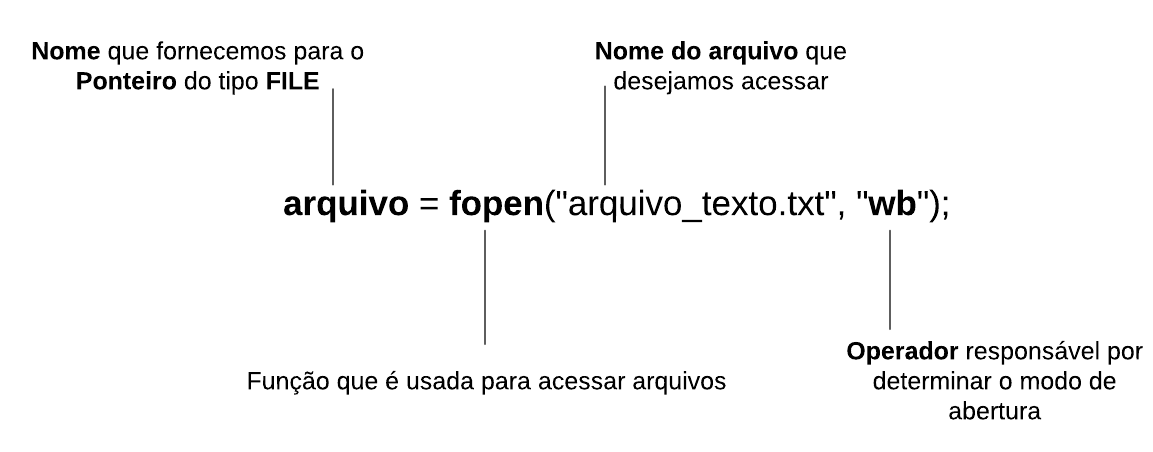
\includegraphics[width=1\linewidth]{figuras/bin.png}
    \end{figure}
\end{frame}

\begin{frame}{Operadores Utilizados para Arquivos Binários}
    \begin{table}[h]
    \centering
    \begin{tabular}{|c|l|}
        \hline
        \textbf{Modo} & \textbf{Descrição} \\
        \hline
        \texttt{"\textbf{rb}"}   & Abre um arquivo para leitura binária.\\
                        & Se o arquivo não existir, retorna \texttt{NULL}. \\
        \hline
        \texttt{"\textbf{wb}"}   & Cria um arquivo para escrita binária. \\
                        & Se o arquivo já existir, ele será apagado. \\
        \hline
        \texttt{"\textbf{ab}"}   & Abre um arquivo para adicionar dados binários no final. \\
                        & Não altera dados existentes no arquivo. \\
        \hline
        \texttt{"\textbf{rb+}"}  & Abre um arquivo para leitura e escrita binária. \\
                        & O arquivo deve existir previamente. \\
        \hline
        \texttt{"\textbf{wb+}"}  & Cria um arquivo para leitura e escrita binária. \\
                        & Se o arquivo já existir, ele será apagado. \\
        \hline
        \texttt{"\textbf{ab+}"}  & Abre um arquivo para leitura e escrita binária. \\
                        & Não apaga dados existentes no arquivo. \\
        \hline
    \end{tabular}
    \caption{Modos de abertura de arquivos binários em C}
    \label{tab:modos_arquivo_binario}
\end{table}
\end{frame}

\begin{frame}{Arquivos Binários}
Acessando um Arquivo Binário:
\begin{figure}
    \centering
    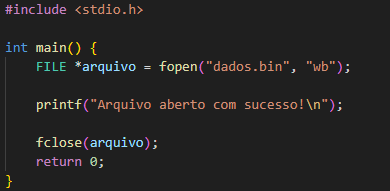
\includegraphics[width=0.75\linewidth]{figuras/bin2.png}
\end{figure}
    
\end{frame}

\begin{frame}{Escrevendo em Arquivos Binários}
\begin{figure}
    \centering
    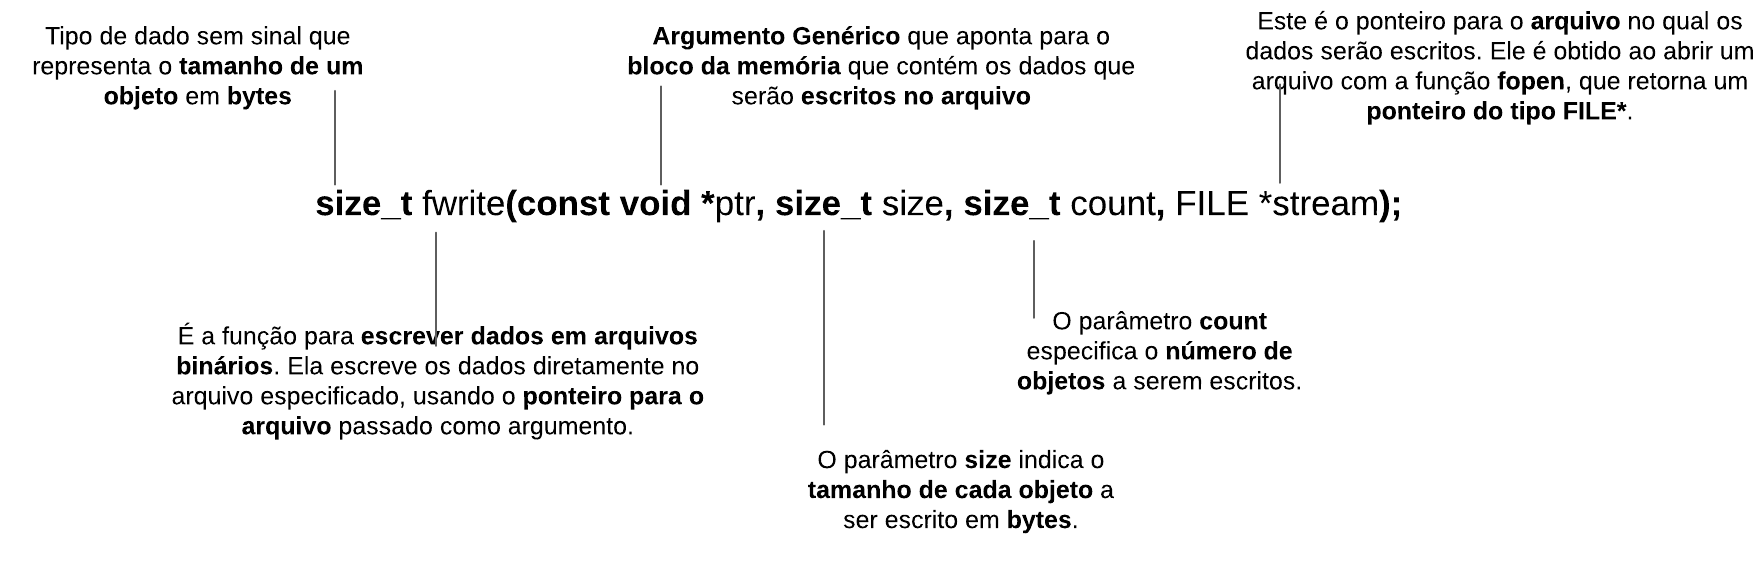
\includegraphics[width=1\linewidth]{figuras/Declarabin.png}
\end{figure}
\end{frame}

\begin{frame}{Escrevendo em Arquivos Binários}
    A manipulação de arquivos binários é feita com registros
\begin{itemize}
    \item O registro se torna o molde usado para gravar e ler informações
\end{itemize}
\begin{figure}
    \centering
    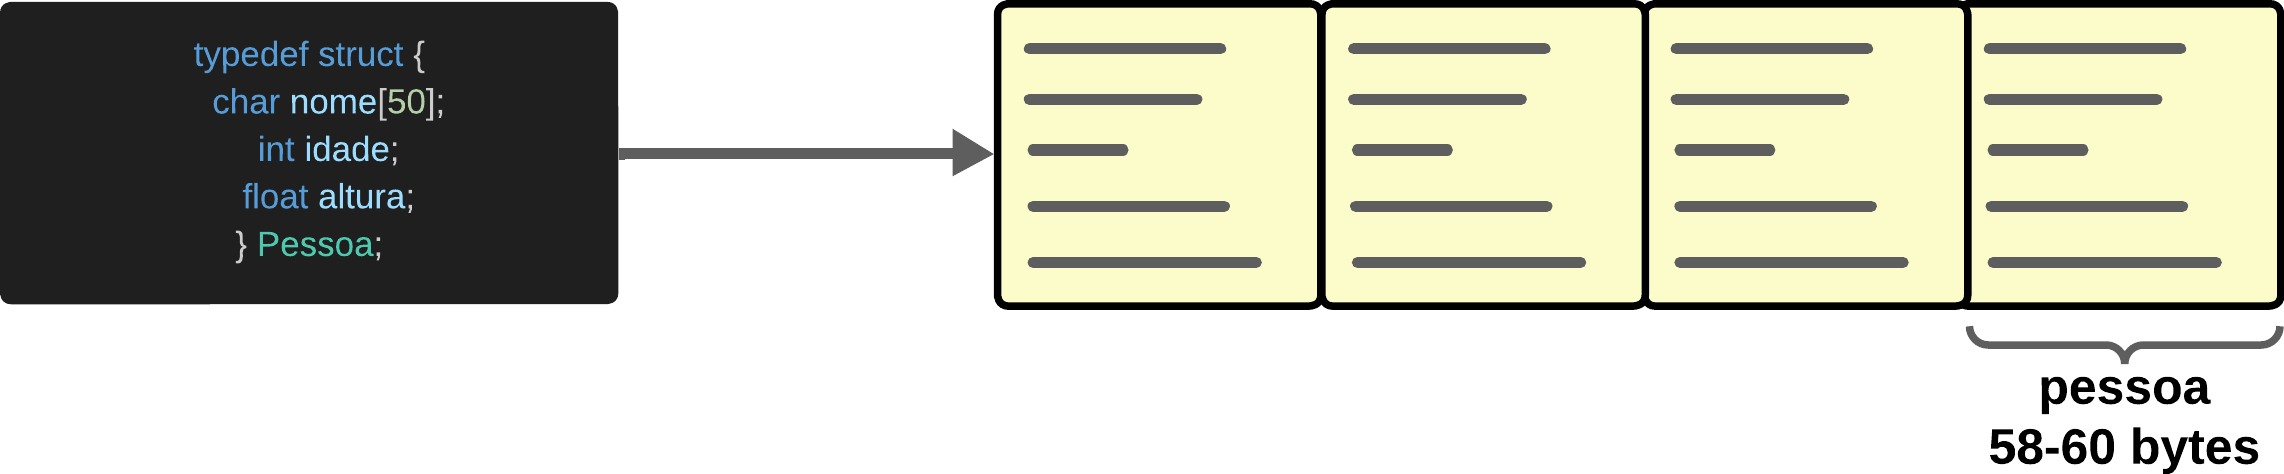
\includegraphics[width=0.75\linewidth]{figuras/binRegs.png}
\end{figure}
\end{frame}


\begin{frame}{Escrevendo em Arquivos Binários}
\begin{figure}
    \centering
    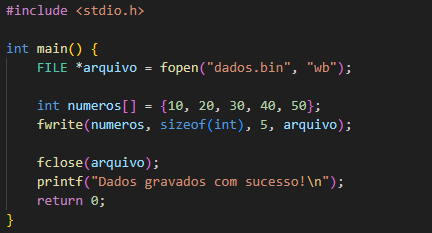
\includegraphics[width=0.75\linewidth]{figuras/binWrite.png}
\end{figure}
    \\Agora vejam como está a escrita desse arquivo na sua máquina...
\end{frame}



\begin{frame}{Movendo-se em Arquivos Binários}
\textbf{Função fseek()}:
    \begin{figure}
        \centering
        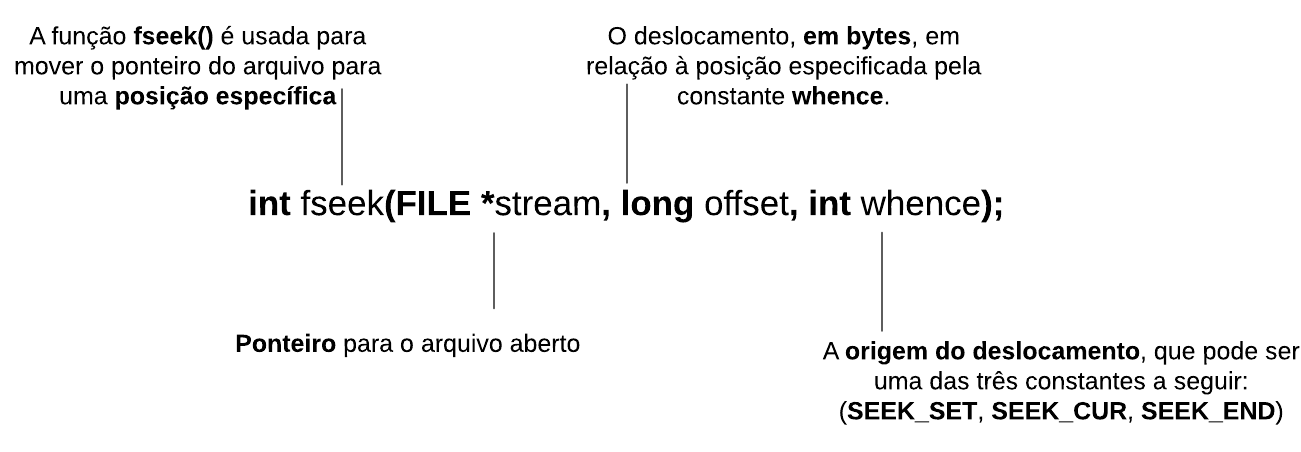
\includegraphics[width=1\linewidth]{figuras/movebin.png}
    \end{figure}

\end{frame}


\begin{frame}{Movendo-se em Arquivos Binários}
    \begin{itemize}
        \item \textbf{SEEK\_SET}: Desloca o ponteiro para a posição relativa ao início do arquivo. O offset será o número de bytes a partir do início do arquivo.
        \item \textbf{SEEK\_CUR}: Desloca o ponteiro para a posição relativa à posição atual. O offset será somado (ou subtraído, se negativo) à posição atual.
        \item \textbf{SEEK\_END}: Desloca o ponteiro para a posição final do arquivo. O offset será adicionado (ou subtraído, se negativo) à posição final do arquivo.
    \end{itemize}
\end{frame}

\begin{frame}{Movendo-se em Arquivos Binários}
\textbf{Função ftell()}:
    \begin{figure}
        \centering
        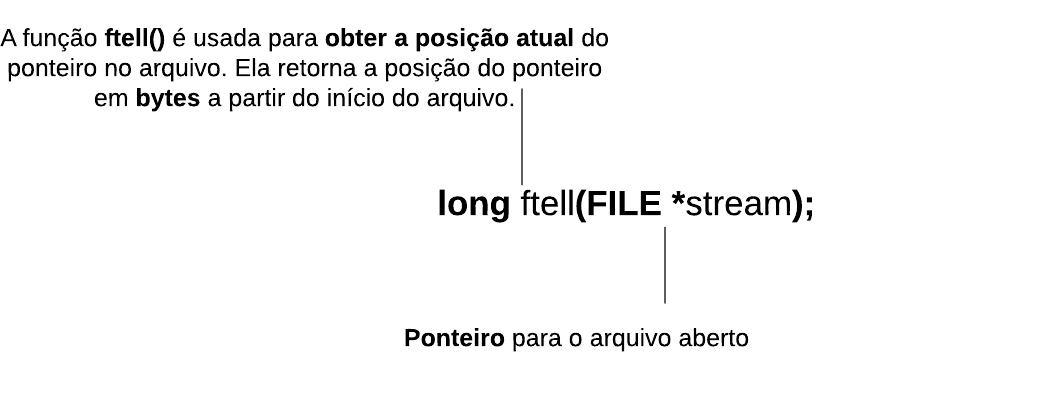
\includegraphics[width=1\linewidth]{figuras/movebin2.png}
    \end{figure}

\end{frame}

\begin{frame}{Movendo-se em Arquivos Binários}
\textbf{Função rewind()}:
    \begin{figure}
        \centering
        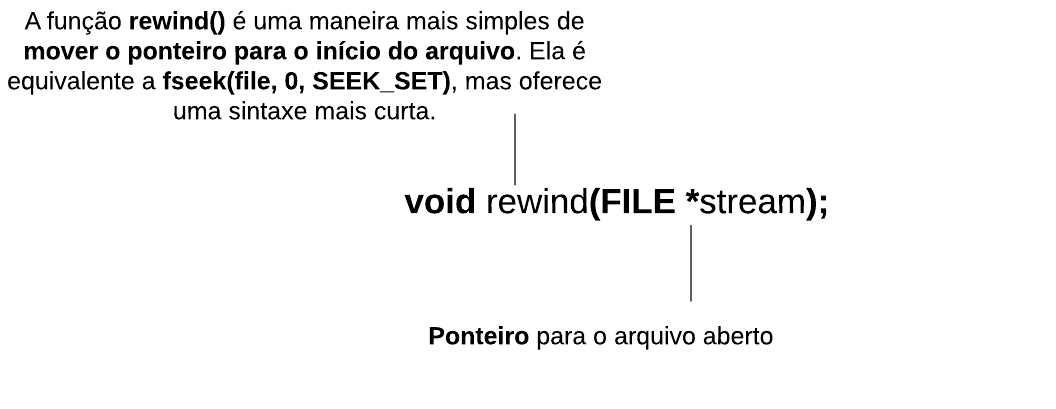
\includegraphics[width=1\linewidth]{figuras/movebin3.png}
    \end{figure}

\end{frame}


\begin{frame}{Lendo em Arquivos Binários}
\begin{figure}
    \centering
    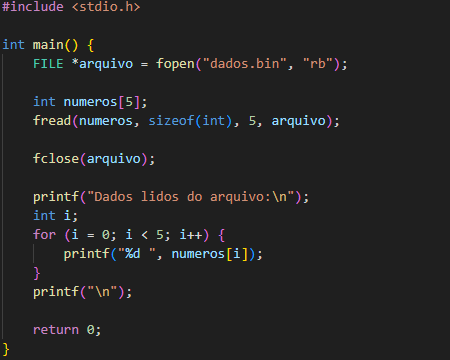
\includegraphics[width=0.75\linewidth]{figuras/binRead.png}
\end{figure}

\end{frame}

\begin{frame}{Alterando Arquivos Binários}
\begin{figure}
    \centering
    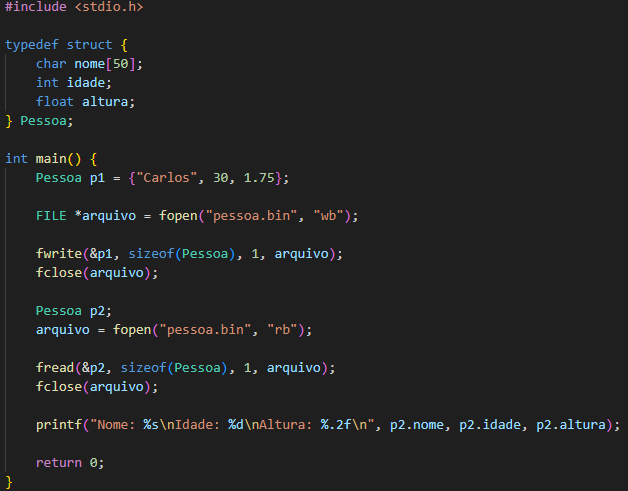
\includegraphics[width=0.75\linewidth]{figuras/binEdit.png}
\end{figure}

\end{frame}

\begin{frame}{Desafio}
\begin{itemize}
    \item Façam um código que \textbf{crie um arquivo binário} e o \textbf{preencham com informações}
    \item Em seguida \textbf{leiam as informações} que vocês preencheram no arquivo
    \item Em seguida \textbf{alterem alguma informação} que vocês preencheram anteriormente
    \item Leiam novamente o \textbf{arquivo atualizado}
\end{itemize}
\end{frame}

\begin{frame}{Desafio}
Trabalhei com funções para separar melhor as etapas do desafio:
\begin{figure}
    \centering
    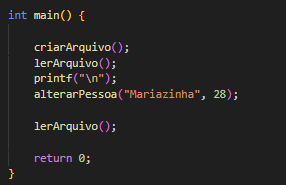
\includegraphics[width=0.5\linewidth]{figuras/Codbin1.png}
\end{figure}
\end{frame}

\begin{frame}{Desafio}
Em seguida criei as funções de criar e ler arquivos:
\begin{figure}
    \centering
    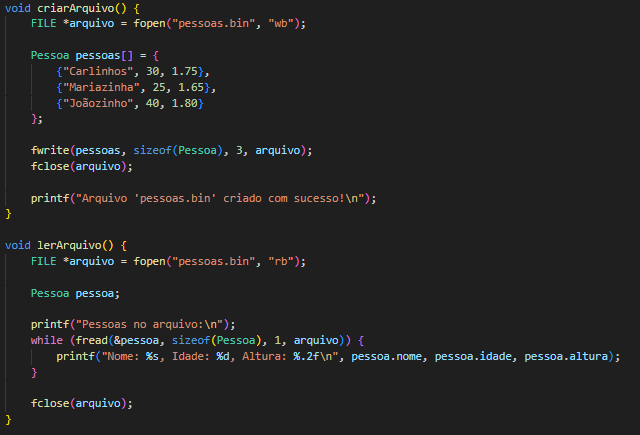
\includegraphics[width=0.75\linewidth]{figuras/Codbin2.png}
\end{figure}
\end{frame}

\begin{frame}{Desafio}
Em seguida criei a função de editar arquivos:
\begin{figure}
    \centering
    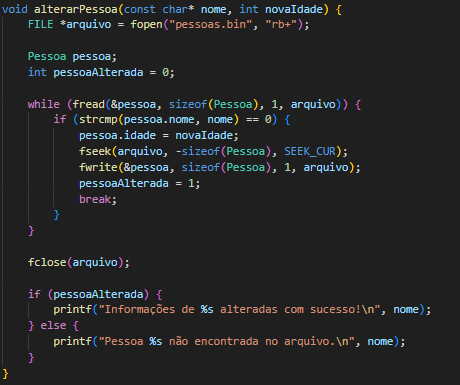
\includegraphics[width=0.75\linewidth]{figuras/Codbin3.png}
\end{figure}
\end{frame}

\section{Conclusão}

\begin{frame}{Resumo}
    Entrada e saída em arquivos é um recurso importante
    \begin{itemize}
        \item Utilizado por praticamente todos os programas
    \end{itemize}
    Os dados podem ser armazenados em:
    \begin{itemize}
        \item \textbf{Arquivos texto}: podem ser lidos por qualquer editor de texto
        \item \textbf{Arquivos binários}: são mais precisos para armazenar números ponto flutuante, as operações de leitura e escrita são mais rápidas, mas
geralmente ocupam mais espaço
    \end{itemize}
\end{frame}

\begin{frame}{Resumo}
    \begin{itemize}
        \item \textbf{Arquivos texto}:
        \begin{itemize}
            \item Podem ser lidos por qualquer editor de texto
            \item Marca de fim de linha (CR[CarriageReturn]/LF[LineFeed]) é diferente para cada S.O.
        \end{itemize}
        \item \textbf{Arquivos binários}:\begin{itemize}
            \item São mais precisos para armazenar números ponto-flutuante
            \item As operações de leitura e escrita são mais rápidas
            \item Geralmente ocupam mais espaço
        \end{itemize}
    \end{itemize}    
\end{frame}